
   \documentclass{standalone}
   \usepackage{tikz}
   %\usetikzlibrary{positioning,shapes}
   \usepackage{pgfplots}
   \begin{document}
   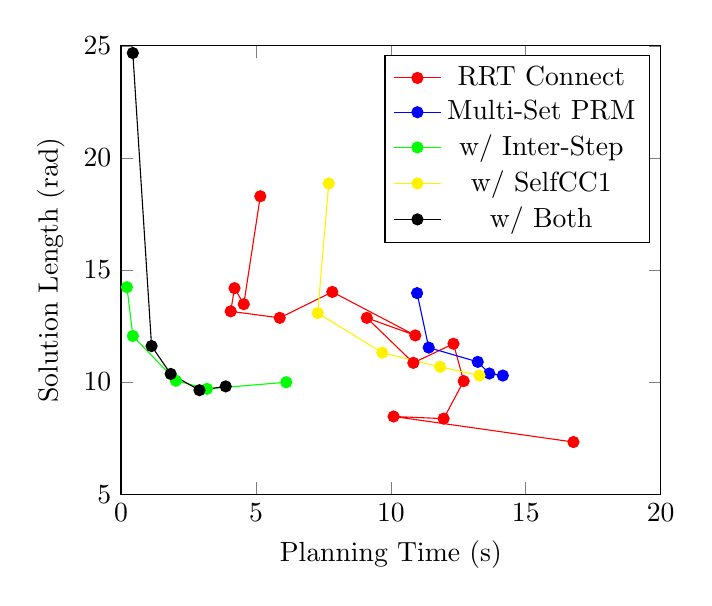
\begin{tikzpicture}
   
   \begin{axis}[
      xlabel=Planning Time (s),
      ylabel=Solution Length (rad),
      ylabel near ticks,
      xlabel near ticks,
      xmin=0,xmax=20,
      ymin=5,ymax=25]
   
   \addplot[mark=*,red] plot coordinates {
     (16.7673695087,7.3242179756)
  (10.102419424,8.46383884964)
  (11.9565801859,8.36755111384)
  (12.7000402927,10.0409246794)
  (12.3211734772,11.7079088994)
  (10.8328934431,10.85582116)
  (9.10966339112,12.8635726876)
  (10.9054726839,12.0799615229)
  (7.83025419713,14.0200152361)
  (5.88109991551,12.8640084226)
  (4.06455712318,13.1553436093)
  (4.20631098747,14.1887453311)
  (4.54932506084,13.4733451222)
  (5.16229887009,18.2881624958)

   };
   \addlegendentry{RRT Connect}
   
   \addplot[mark=*,blue] plot coordinates {
     (14.1501514196,10.2897866493)
  (13.6496914864,10.381351282)
  (13.2208489656,10.8997604855)
  (11.4035658598,11.5373957412)
  (10.9726590395,13.966562752)

   };
   \addlegendentry{Multi-Set PRM}
   
   \addplot[mark=*,green] plot coordinates {
     (6.12460656166,9.99059870969)
  (3.18511879444,9.69637537219)
  (2.03236260414,10.0608947001)
  (0.439556241035,12.0559928329)
  (0.218989872932,14.2331896569)

   };
   \addlegendentry{w/ Inter-Step}
   
   \addplot[mark=*,yellow] plot coordinates {
     (13.2860650301,10.2897866493)
  (11.82657938,10.6762625474)
  (9.68265879154,11.3103554892)
  (7.28945250511,13.0783571525)
  (7.69926218987,18.8603466704)

   };
   \addlegendentry{w/ SelfCC1}
   
   \addplot[mark=*,black] plot coordinates {
     (3.88056988186,9.80592991052)
  (2.90637376573,9.63593870284)
  (1.83979598681,10.3626999827)
  (1.13230668174,11.6060333762)
  (0.436946868897,24.6777786523)

   };
   \addlegendentry{w/ Both}
   
   \end{axis}
   
   \end{tikzpicture}
   \end{document}
   